\chapter{Budowa modeli}

\section{Jednowarstwowa architektura LSTM}

\ref{rys:lstm_one_graph} rysunek przedstawiający budowę jednowarstwowej architektury LSTM.

\begin{figure}[t]
\centering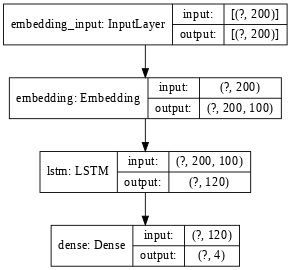
\includegraphics[width=6cm]{figures/reports/lstm_one_graph.png}
\fcmfcaption{Graf przedstawiający budowę jednowarstwowej architektury LSTM.}\label{rys:lstm_one_graph}
\end{figure}

\ref{rys:lstm_one_table} tabela przedstawiająca szczegóły budowy jednowarstwowej architektury LSTM.

\begin{figure}[t]
\centering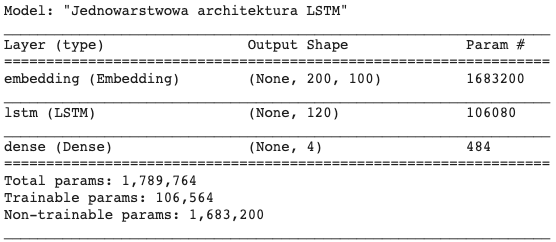
\includegraphics[width=10cm]{figures/reports/lstm_one_table.png}
\fcmfcaption{Tabela przedstawiająca szczegóły budowy jednowarstwowej architektury LSTM.}\label{rys:lstm_one_table}
\end{figure}

\section{Głęboka architektura LSTM}

\ref{rys:lstm_deep_graph} graf głębokiej architektury LSTM

\begin{figure}[t]
\centering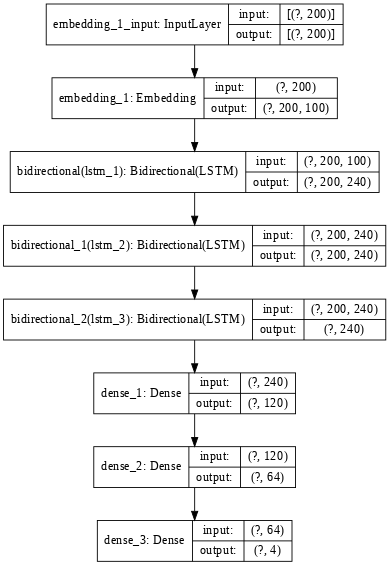
\includegraphics[width=8cm]{figures/reports/lstm_deep_graph.png}
\fcmfcaption{Graf przedstawiający budowę głębokiej architektury LSTM.}\label{rys:lstm_deep_graph}
\end{figure}

\ref{rys:lstm_deep_table} tabela przedstawiająca szczegóły budowy głębokiej architektury LSTM.

\begin{figure}[t]
\centering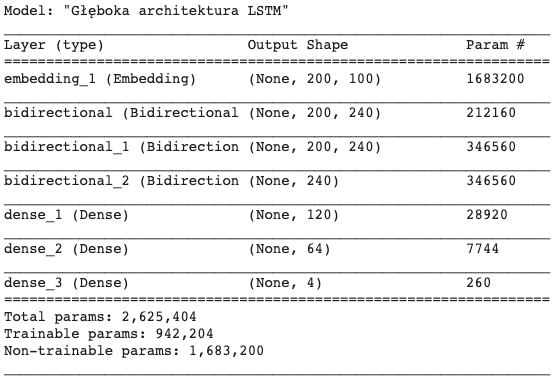
\includegraphics[width=10cm]{figures/reports/lstm_deep_table.png}
\fcmfcaption{Tabela przedstawiająca szczegóły budowy głębokiej architektury LSTM.}\label{rys:lstm_deep_table}
\end{figure}

\cite{brochier2019global} GLOVE

\section{Głęboka architektura BERT}

\cite{devlin2018bert} BERT

\section{Porównanie budowy modeli}

\begin{table}[t]
\fcmtcaption{Tabela porównująca szczegóły budowy poszczególnych model.}\label{tab:tabela_modele}
\centering\footnotesize%
\begin{tabular}{c c c c}
\toprule
model & parametry trenowalne & parametry stałe & SUMA \\
\midrule
Jednowarstwowy LSTM   & 106,564 & 1,683,200 & 1,789,764 \\
Głęboki LSTM   & 942,204 & 1,683,200 & 2,625,404 \\
BERT todo   & xx & xx & xxx \\
\bottomrule
\end{tabular}
\end{table}